\pretextual


% ---
% Folha de rosto
% (o * indica que haverá a ficha bibliográfica e deverá ser usado para teses 
%   e dissertações. Para projetos, favor retirar o *)
% ---
\imprimirfolhaderosto*
% ---

% ---
% Inserir a ficha bibliografica
% ---

%  A ficha catalografica, preparada pela biblioteca do departamento de física da UFMG é
% um elemento obrigatório para teses e dissertações. Inclua o arquivo pdf fornecido de acordo
% com o comando abaixo, modificando o nome e a localização do arquivo quando necessário.
%
\begin{fichacatalografica}
    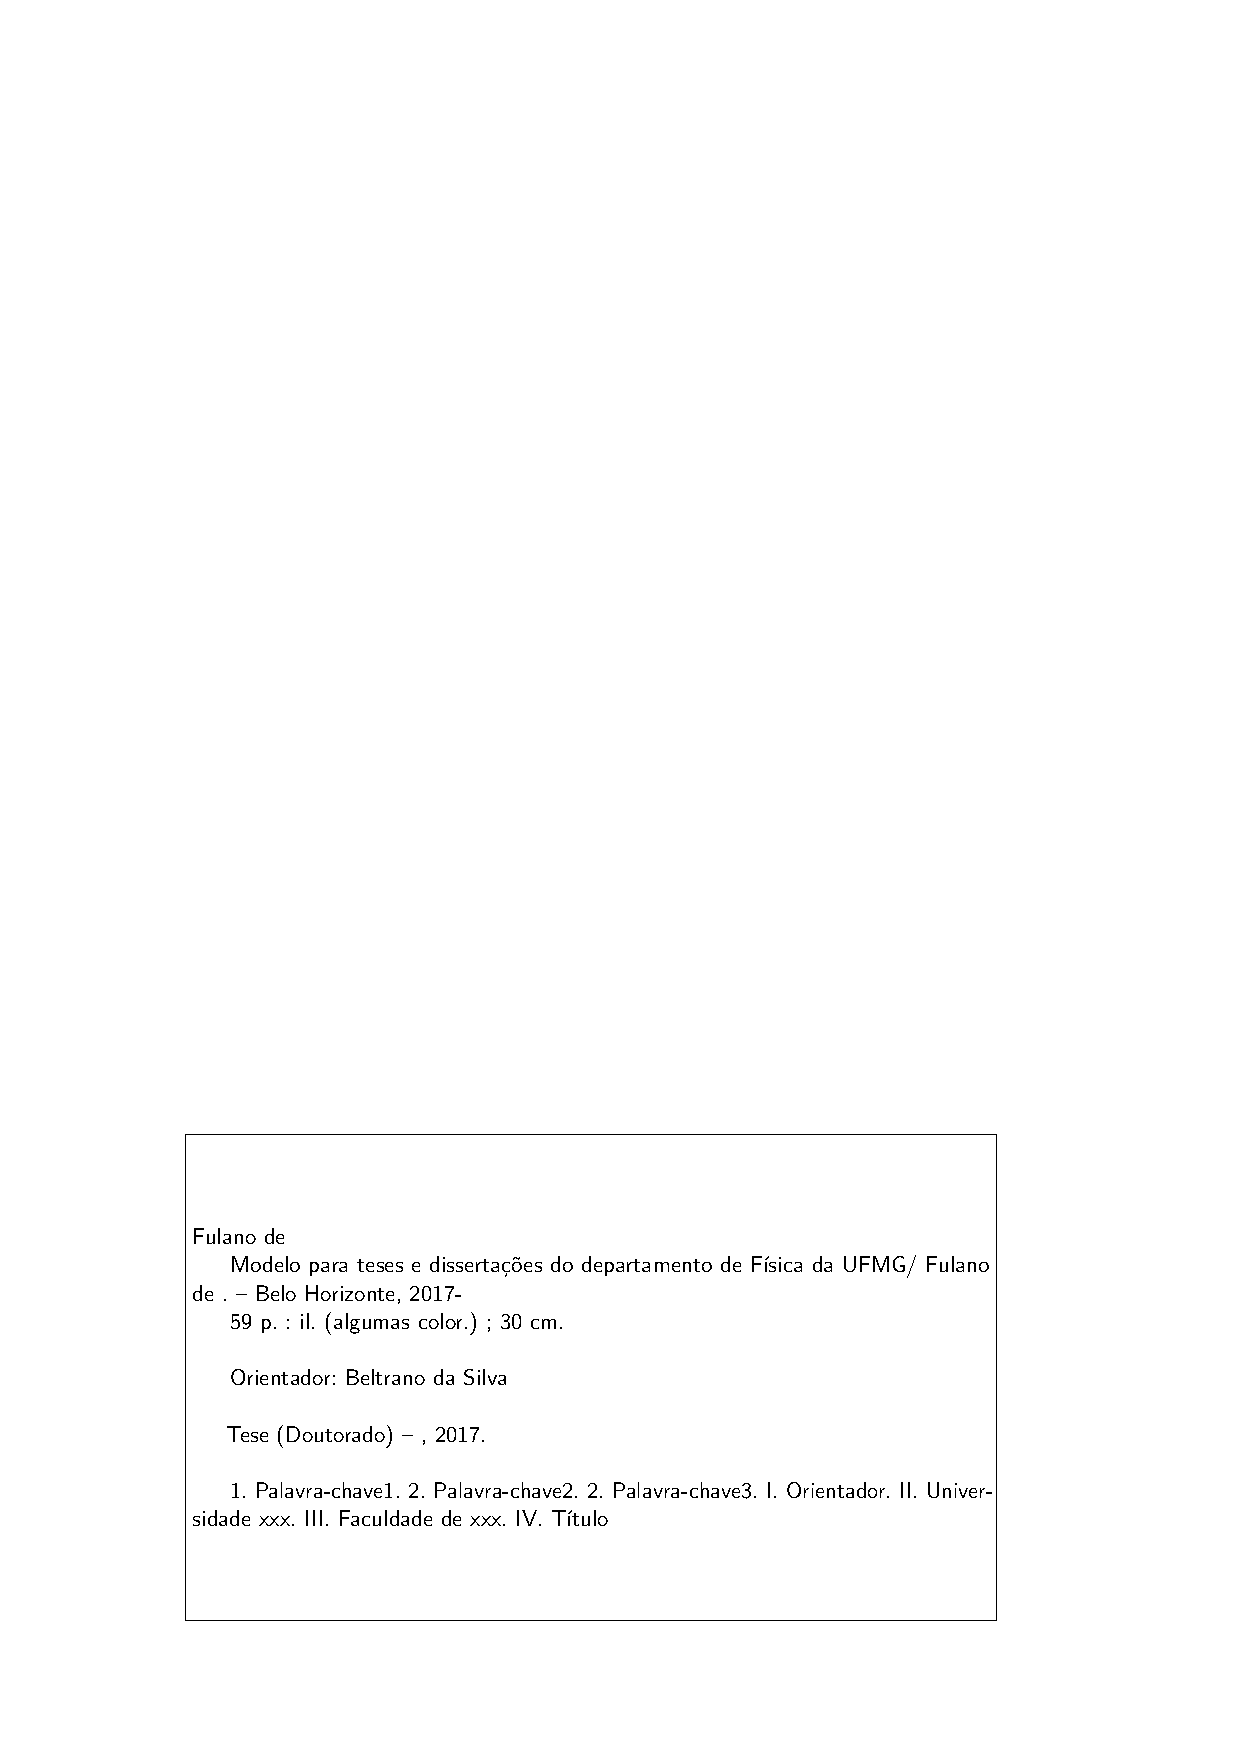
\includepdf{fig/ficha-catalografica.pdf}
\end{fichacatalografica}

% ---
% Inserir folha de aprovação
% ---

% A folha de aprovação é um elemento obrigatório da versão final do trabalho e deverá ser incluído
% conforme comando abaixo.
%
% TODO: na versao final incluir a ficha de aprovacao
\begin{folhadeaprovacao}
     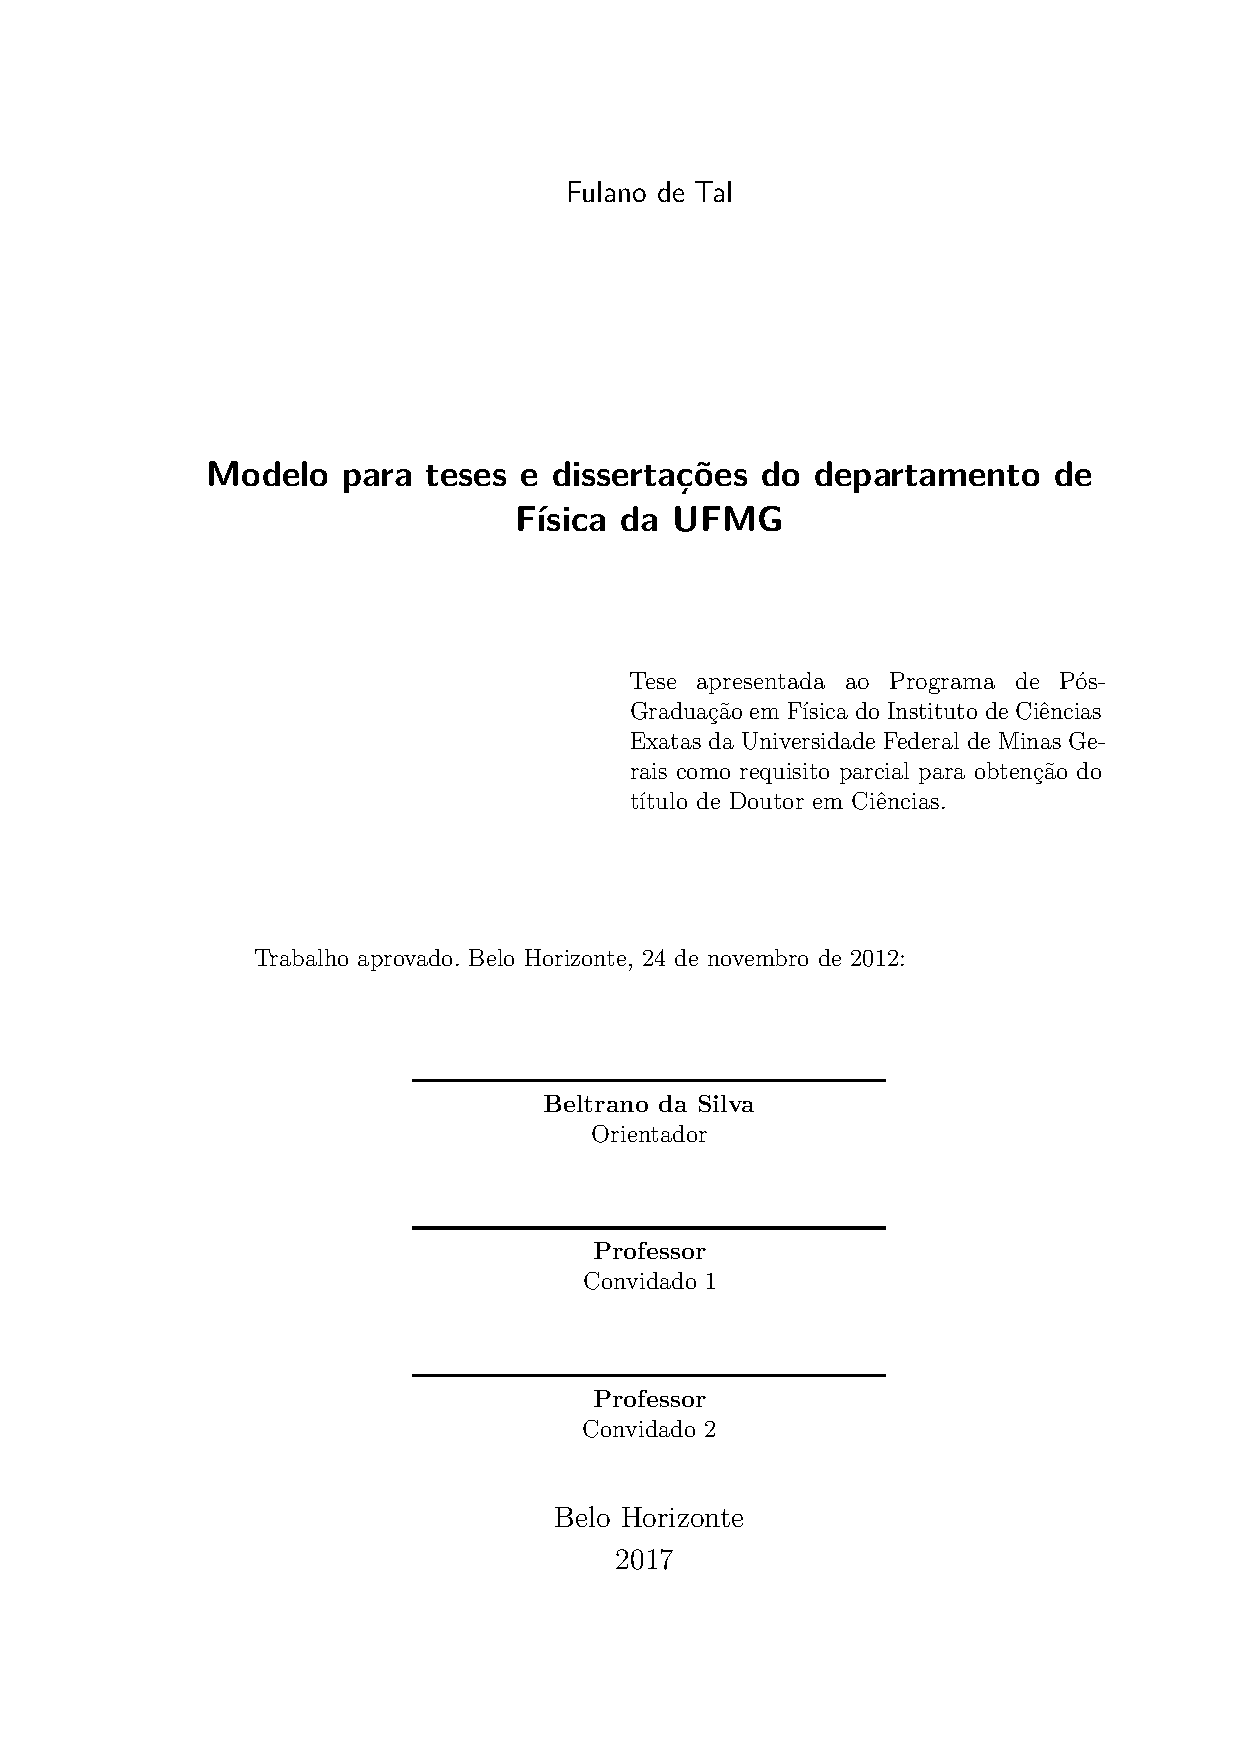
\includepdf{fig/folhadeaprovacao.pdf}
\end{folhadeaprovacao}
%


% ---
% Dedicatória - OPCIONAL
% ---
%\begin{dedicatoria}
%   \vspace*{\fill}
%   \centering
%   \noindent
%   \textit{\textbf{Dedicatória. Elemento opcional. Não há formatação a ser seguida.}\\
%    Este trabalho é dedicado às crianças adultas que,\\
%   quando pequenas, sonharam em se tornar cientistas.} \vspace*{\fill}
%\end{dedicatoria}
% ---

% ---
% Agradecimentos
% ---
\begin{agradecimentos}
Os agradecimentos são obrigatórios para os bolsistas e opcional para os demais. 
\end{agradecimentos}
% ---

% ---
% Epígrafe - OPCIONAL
% ---
%\begin{epigrafe}
%    \vspace*{\fill}
%	\begin{flushright}
%		\textit{\textbf{Epígrafe. Elemento opcional. Não há formatação a ser seguida.}\\
%		``Não vos amoldeis às estruturas deste mundo, \\
%		mas transformai-vos pela renovação da mente, \\
%		a fim de distinguir qual é a vontade de Deus: \\
%		o que é bom, o que Lhe é agradável, o que é perfeito.\\
%		(Bíblia Sagrada, Romanos 12, 2)}
%	\end{flushright}
%\end{epigrafe}
% ---

% ---
% RESUMOS
% ---

% resumo em português
\setlength{\absparsep}{18pt} % ajusta o espaçamento dos parágrafos do resumo
\begin{resumo}
\begin{otherlanguage*}{brazil}
O Resumo em português é um elemento obrigatório. Consiste de uma síntese de pontos relevantes com apresentação do objetivo, métodos,
técnicas, resultados e conclusões. Deve apresentar, abaixo, as palavras-chave relacionadas ao trabalho. Não pode exceder uma página.

\vspace{\onelineskip}
 
\noindent 
 \textbf{Palavras-chave}: Modelo, Tese, Dissertação, Projeto
\end{otherlanguage*}{brazil}

\end{resumo}

% resumo em inglês
\begin{resumo}[Abstract]
%\begin{otherlanguage*}{english}
The abstract and keywords, in English, are also mandatory and must fit in one page.
\vspace{\onelineskip}
 
\noindent 
\textbf{Keywords}: Template, Dissertations, Thesis, Projects.
%\end{otherlanguage*}

\end{resumo}

% ---
% LISTAS - CONTEÚDO DE CARÁTER OPCIONAL
% ---
% ---
% AS LISTAS DE ILUSTRAÇÕES, TABELAS, ABREVIATURAS E SIGLAS E SÍMBOLOS SÃO ELEMENTOS OPCIONAIS.
% RESSALTA-SE A IMPORTÂNCIA DE SE AO UTILIZAR TAIS LISTAS INCLUIR CORRETAMENTE NO LATEX UM TÍTULO
% PARA CADA FIGURA OU TABELA AO INVÉS DE DEIXAR A LEGENDA COMPLETA, QUE É, EM GERAL, MUITO GRANDE
% E POUCO INSTRUTIVA. ISTO É FEITO COM O SEGUINTE COMANDO: \caption[título da figura]{Legenda da figura}
% ---

% ---
% inserir lista de ilustrações - OPCIONAL
% ---
%\pdfbookmark[0]{\listfigurename}{lof}
%\listoffigures*
%\cleardoublepage
% ---

% ---
% inserir lista de tabelas - OPCIONAL
% ---
%\pdfbookmark[0]{\listtablename}{lot}
%\listoftables*
%\cleardoublepage
% ---

% ---
% inserir lista de abreviaturas e siglas - OPCIONAL
% ---
%\begin{siglas}
%  \item[ABNT] Associação Brasileira de Normas Técnicas
%  \item[abnTeX] ABsurdas Normas para TeX
%\end{siglas}
% ---

% ---
% inserir lista de símbolos - OPCIONAL
% ---
%\begin{simbolos}
%  \item[$ \Gamma $] Letra grega Gama
%  \item[$ \Lambda $] Lambda
%  \item[$ \zeta $] Letra grega minúscula zeta
%  \item[$ \in $] Pertence
%\end{simbolos}
% ---



% ---
% O SUMARIO É OBRIGATÓRIO
% ---

% ---
% inserir o sumario
% ---
\pdfbookmark[0]{\contentsname}{toc}
\tableofcontents*
\cleardoublepage
% ---


